\documentclass[a4paper,12pt]{article}

\usepackage{graphicx} % Required for inserting images
\usepackage{amsmath,amssymb,amsfonts}
\usepackage{subcaption}
% -----------------------
% Package Imports
% -----------------------

% Set page margins
\usepackage[a4paper, top=1in, bottom=0.8in, left=1.1in, right=0.8in]{geometry}

% Use Times New Roman font
\usepackage{times}

% Add page numbering
\pagestyle{plain}
\usepackage{multirow}
% Enable graphics inclusion
\usepackage{graphicx}
\usepackage{float}
% Enable code listings
\usepackage{listings}
\usepackage{xcolor} % For customizing code colors
% -----------------------
% Section Font Customization
% -----------------------
\usepackage{titlesec} % To customize section font size
\titleformat{\section}
{\normalfont\fontsize{14}{16}\bfseries}{\thesection}{1em}{}

\titleformat{\subsection}
{\normalfont\fontsize{14}{16}\bfseries}{\thesubsection}{1em}{}


\definecolor{codegreen}{rgb}{0,0.6,0}
\definecolor{codegray}{rgb}{0.5,0.5,0.5}
\definecolor{codepurple}{rgb}{0.58,0,0.82}
\definecolor{backcolour}{rgb}{0.98,0.98,0.98}

\lstdefinestyle{mystyle}{
	backgroundcolor=\color{backcolour},
	commentstyle=\color{codegreen},
	keywordstyle=\color{magenta},
	numberstyle=\tiny\color{codegray},
	stringstyle=\color{codepurple},
	basicstyle=\ttfamily\footnotesize,
	breakatwhitespace=false,
	breaklines=true,
	captionpos=b,
	keepspaces=true,
	numbers=left,
	numbersep=5pt,
	showspaces=false,
	showstringspaces=false,
	showtabs=false,
	tabsize=2
}

\lstset{style=mystyle}

\setlength{\parindent}{0pt}


\begin{document}
	\section{Experiment No. 10}
	
	\section{Experiment Title }
	Solving ordinary differential equations using various numerical methods (Euler’s Method, Heun’s Method, Modified Euler’s/Runge Kutta 2nd Order Method, Runge Kutta 4th Order Method)
	\section{Objective}
	
	The objectives of this lab are:
	\begin{itemize}
		\item To gather knowledge about different types of step-by-step numerical methods of solving ordinary differential equation..
		\item To know the methods of solving ODE using Euler’s method, modified Euler’s method and Runge-Kutta methods.
	\end{itemize}
	\section*{Theory}
	
	Ordinary Differential Equations (ODEs) are equations that involve functions of one independent variable and their derivatives. Numerical methods are often used to approximate solutions of ODEs when analytical methods are difficult or impossible to apply.
	
	We consider the first-order ODE:
	\[
	\frac{dy}{dx} = f(x, y) = 4e^{0.8x} - 0.5y
	\]
	
	The following numerical methods are used to solve this equation:
	
	\subsection*{Euler’s Method}
	Euler’s method is the simplest numerical approach based on the Taylor series expansion. It estimates the next value using the slope at the current point:
	\[
	y_{n+1} = y_n + h f(x_n, y_n)
	\]
	where \( h \) is the step size. This method may accumulate error over large intervals due to its first-order accuracy.
	
	\subsection*{Heun’s Method}
	Heun’s method (Improved Euler method) uses a predictor-corrector approach. First, it predicts the value using Euler’s method and then corrects it using the average of the slopes at the beginning and end of the interval:
	\[
	y_{k+1} = y_k + \frac{h}{2} \left[f(x_k, y_k) + f(x_{k+1}, y_{k+1})\right]
	\]
	
	\subsection*{Modified Euler’s / Runge-Kutta 2nd Order Method}
	This method also improves upon Euler’s method by estimating the slope at the midpoint of the interval:
	\begin{align*}
		f_1 &= f(x_k, y_k) \\
		f_2 &= f\left(x_k + \frac{h}{2}, y_k + \frac{h}{2}f_1\right) \\
		y_{k+1} &= y_k + h f_2
	\end{align*}
	
	\subsection*{Runge-Kutta 4th Order Method}
	The RK4 method is one of the most widely used techniques due to its high accuracy. It calculates four slopes and combines them to estimate the next value:
	\begin{align*}
		f_1 &= f(x_k, y_k) \\
		f_2 &= f\left(x_k + \frac{h}{2}, y_k + \frac{h}{2} f_1\right) \\
		f_3 &= f\left(x_k + \frac{h}{2}, y_k + \frac{h}{2} f_2\right) \\
		f_4 &= f(x_k + h, y_k + h f_3) \\
		y_{k+1} &= y_k + \frac{h}{6} (f_1 + 2f_2 + 2f_3 + f_4)
	\end{align*}
	
	\section*{Algorithm}
	
	\subsection*{Step 1: Define the differential equation and initial conditions}
	\begin{itemize}
		\item Define the function: \( f(x, y) = 4e^{0.8x} - 0.5y \)
		\item Set initial conditions:
		\begin{itemize}
			\item \( x_0 = 0 \)
			\item \( y_0 = 1 \)
		\end{itemize}
		\item Define step size: \( h = 0.5 \)
		\item Define final value: \( x_n = 5 \)
		\item Compute number of steps: \( n = \frac{x_n - x_0}{h} \)
	\end{itemize}
	
	\subsection*{Step 2: Initialize arrays for x and y}
	\begin{itemize}
		\item Create array \( x[] \) of size \( n+1 \) to store x-values.
		\item Create array \( y[] \) of size \( n+1 \) to store y-values.
		\item Set initial values:
		\begin{itemize}
			\item \( x[1] = x_0 \)
			\item \( y[1] = y_0 \)
		\end{itemize}
	\end{itemize}
	
	\subsection*{Step 3: Implement Numerical Methods}
	
	\paragraph{Euler's Method}
	\begin{itemize}
		\item For \( i = 1 \) to \( n \):
		\begin{itemize}
			\item \( x[i+1] = x[i] + h \)
			\item \( y[i+1] = y[i] + h \cdot f(x[i], y[i]) \)
		\end{itemize}
	\end{itemize}
	
	\paragraph{Heun's Method (Modified Euler)}
	\begin{itemize}
		\item For \( i = 1 \) to \( n \):
		\begin{itemize}
			\item \( x[i+1] = x[i] + h \)
			\item Predictor: \( y_{\text{pred}} = y[i] + h \cdot f(x[i], y[i]) \)
			\item Corrector: \( y[i+1] = y[i] + \frac{h}{2} \cdot \left(f(x[i], y[i]) + f(x[i+1], y_{\text{pred}})\right) \)
		\end{itemize}
	\end{itemize}
	
	\paragraph{Runge-Kutta 2nd Order Method}
	\begin{itemize}
		\item For \( i = 1 \) to \( n \):
		\begin{itemize}
			\item \( f_1 = f(x[i], y[i]) \)
			\item \( f_2 = f\left(x[i] + \frac{h}{2}, y[i] + \frac{h}{2} f_1\right) \)
			\item \( y[i+1] = y[i] + h \cdot f_2 \)
		\end{itemize}
	\end{itemize}
	
	\paragraph{Runge-Kutta 4th Order Method}
	\begin{itemize}
		\item For \( i = 1 \) to \( n \):
		\begin{itemize}
			\item \( f_1 = f(x[i], y[i]) \)
			\item \( f_2 = f\left(x[i] + \frac{h}{2}, y[i] + \frac{h}{2} f_1\right) \)
			\item \( f_3 = f\left(x[i] + \frac{h}{2}, y[i] + \frac{h}{2} f_2\right) \)
			\item \( f_4 = f(x[i] + h, y[i] + h f_3) \)
			\item \( y[i+1] = y[i] + \frac{h}{6} (f_1 + 2f_2 + 2f_3 + f_4) \)
		\end{itemize}
	\end{itemize}
	
	\paragraph{Analytical Solution}
	\begin{itemize}
		\item The exact solution of the differential equation is given by:
		\[
		y(x) = \frac{40}{13} e^{0.8x} - 2.0769 e^{-0.5x}
		\]
	\end{itemize}
	
	\subsection*{Step 4: Plot the Results}
	\begin{itemize}
		\item Plot all numerical methods and the analytical solution on the same graph.
		\item Add a legend to distinguish each method clearly.
	\end{itemize}
	
	
	\newpage
	\subsection{MATLAB Code for Solving ODE Using Euler, Heunn, RK2, and RK4 Methods}
	
	\subsubsection{MATLAB Code:}
\begin{lstlisting}[language=Matlab, caption=MATLAB Code for Solving ODE using different Methods]
	clc;
		clc;
		clear;
		f = @(x, y) 4 * exp(0.8 * x) - 0.5 * y;
		
		x0 = 0;
		y0 = 1;
		h = 0.5;
		xn = 5;
		n = (xn - x0) / h
		x = zeros(1, n + 1);
		x(1) = x0;
		y_euler = zeros(1, n + 1);
		y_heun = zeros(1, n + 1);
		y_true = zeros(1, n + 1);
		y_rk2 = zeros(1, n + 1);
		y_rk4 = zeros(1,n+1);
	
		y_euler(1) = y0;
		y_heun(1) = y0;
		y_rk2(1) = y0;
		y_rk4(1) = y0;
		y_exact = @(x) (40 / 13) * exp(0.8 * x) - 2.0769 * exp(-0.5 * x);
		y_true(1) = y_exact(x0);
		
		for i = 1:n
		x(i + 1) = x(i) + h;
		y_true(i + 1) = y_exact(x(i + 1));
		
		y_euler(i + 1) = y_euler(i) + h * f(x(i), y_euler(i));
	
		y_pr = y_heun(i) + h * f(x(i), y_heun(i));
		y_heun(i + 1) = y_heun(i) + (h / 2) * (f(x(i), y_heun(i)) + f(x(i + 1), y_pr));
		
		f1 = f(x(i), y_rk2(i));
		f2 = f(x(i) + h / 2, y_rk2(i) + (h / 2) * f1);
		y_rk2(i + 1) = y_rk2(i) + h * f2;
		
		k1 = f(x(i), y_rk4(i));
		k2 = f(x(i) + h / 2, y_rk4(i) + (h / 2) * k1);
		k3 = f(x(i) + h / 2, y_rk4(i) + (h / 2) * k2);
		k4 = f(x(i) + h, y_rk4(i) + h * k3);
		y_rk4(i + 1) = y_rk4(i) + (h / 6) * (k1 + 2 * k2 + 2 * k3 + k4);
		end
		% Plot 
		figure;
		hold on;
		p1 = plot(x, y_true, '-k.', 'MarkerSize', 20, 'LineWidth', 2);          
		p2 = plot(x, y_euler, '-r.', 'MarkerSize', 10, 'LineWidth', 2);        
		p3 = plot(x, y_heun, '-g.', 'MarkerSize', 10, 'LineWidth', 2);         
		p4 = plot(x, y_rk2, '-b.', 'MarkerSize', 10, 'LineWidth', 2);          
		p5 = plot(x, y_rk4, '-m.', 'MarkerSize', 10, 'LineWidth', 2);          
		xlabel('X- axis');
		ylabel('Y- axis');
		legend([p2 p3 p4 p5 p1], {'Euler Approximation', 'Heun Approximation', ...
			'RK 2nd order', 'RK 4th order', 'Analytical'}, ...
		'Location', 'northwest');
		grid on;
		inset = axes('Position', [0.2 0.3 0.3 0.3]);
		box on; hold on;
		plot(x, y_euler, '-r.', 'MarkerSize', 10, 'LineWidth', 2);
		plot(x, y_heun, '-g.', 'MarkerSize', 10, 'LineWidth', 2);
		plot(x, y_rk2, '-b.', 'MarkerSize', 10, 'LineWidth', 2);
		plot(x, y_rk4, '-m.', 'MarkerSize', 10, 'LineWidth', 2);
		plot(x, y_true, '-k.', 'MarkerSize', 15, 'LineWidth', 2);
		xlim([4.995 5.001]);
		ylim([167 173]);
	\end{lstlisting}
	

	
	
	\subsection{Output}
	
	
	\subsubsection{Plot Diagram}
	\begin{figure}[H]
		\centering
	
		\begin{subfigure}[t]{1\textwidth}
			\centering
				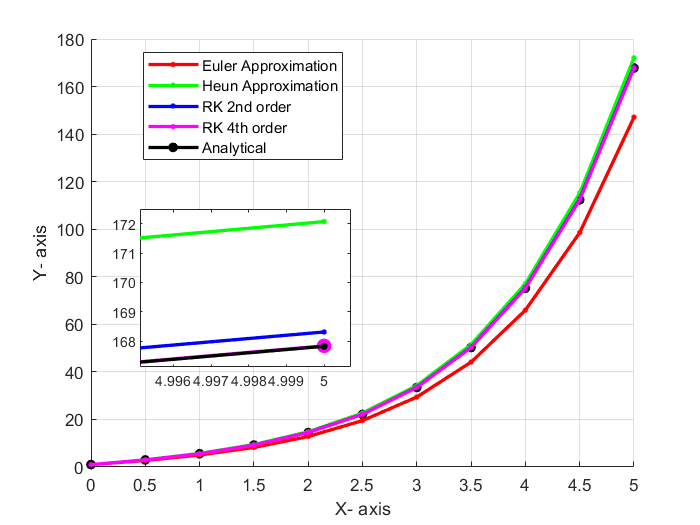
\includegraphics[width=0.81\linewidth]{Images/3}
			\caption{Comparison of numerical methods (Euler, Heun, RK2, RK4) with the analytical solution for the ODE \(\frac{dy}{dx} = 4e^{0.8x} - 0.5y\). The inset plot shows a zoomed-in region near \(x = 5\).}
		\end{subfigure}
		
	\caption{Plot diagram for Solving ODE using different Methods.}
	
	\end{figure}
	\newpage
	\section{Discussion}
	
	In this experiment, several numerical methods were used to solve the differential equation \(\frac{dy}{dx} = 4e^{0.8x} - 0.5y\). Euler’s, Heun’s, Runge-Kutta 2nd order, and Runge-Kutta 4th order methods were implemented in MATLAB and compared with the analytical solution.
	
	Euler’s method gave the least accurate result, especially near \(x = 5\), due to its simple approximation. Heun’s method improved the result slightly by using a correction step. The Runge-Kutta 2nd order method gave better accuracy by considering the midpoint slope.
	
	The most accurate results were obtained using the Runge-Kutta 4th order method, which closely matched the analytical solution throughout. A zoomed-in view near the final point showed that RK4 had the smallest error, while Euler and Heun methods deviated more.
	
	Overall, it was observed that higher-order methods provided better accuracy, with RK4 performing the best among all.
	
\end{document}